\id{IRSTI 65.63.33}

\begin{articleheader}
\sectionwithauthors{N. Alzhaxina, I. Aubakirova }{bfseries OPTIMIZATION OF THE FORMULATION OF VEGETABLE MILK WITH THE
ADDITION OF LEGUMES ON THE EXAMPLE OF MUNG BEAN}

{\bfseries \textsuperscript{1}N. Alzhaxina\textsuperscript{\envelope },
\textsuperscript{1}I. Aubakirova}
\end{articleheader}

\begin{affiliation}
\textsuperscript{1}Astana branch «Kazakh research institute of
processing and food industry» LTD, Astana, Kazakhstan

\raggedright {\bfseries \textsuperscript{\envelope }}Corresponding-author: \href{mailto:alzhaxina@inbox.ru}{\nolinkurl{alzhaxina@inbox.ru}}
\end{affiliation}

One of the key positions of food security is "improving the health of
the population" as the most complete satisfaction of human needs for
basic nutrients - proteins, fats, carbohydrates, vitamins, minerals. A
balanced diet has a huge impact on all aspects of the human
body' s vital activity. Continuously occurring life
processes are impossible without the introduction of nutrients from the
outside. Nowadays, human nutrition is of particular importance precisely
during illness. This study is aimed at developing a functional drink
based on vegetable "milk" using different ratios of mung bean, water and
stabilizer. The results obtained made it possible to select the
formulation of vegetable milk from mung bean by applying the developed
mathematical model. One of the most important indicators of milk quality
is acidity, which characterizes the freshness of milk, its suitability
for further processing and pasteurization. The article describes the
results of fitting various models to the acidity data of vegetable milk.
An increase in acidity leads to the fact that proteins become less
resistant to heat. A model in three-dimensional space is also presented,
characterizing the dependence of acidity on the components of vegetable
milk.

{\bfseries Keywords:} formulation, optimization, vegetable milk, legume
culture, mung bean, acidity, functional purpose.

\begin{articleheader}
{\bfseries МАШ ДАҚЫЛЫ МЫСАЛЫНДА БҰРШАҚ ДАҚЫЛДАРЫН ҚОСУ АРҚЫЛЫ ӨСІМДІК
СҮТІНІҢ РЕЦЕПТУРАСЫН ОҢТАЙЛАНДЫРУ}

{\bfseries \textsuperscript{1}Н.E. Альжаксина\textsuperscript{\envelope },
\textsuperscript{1}И.Е. Аубакирова}
\end{articleheader}

\begin{affiliation}
\textsuperscript{1}Астана филиалы ЖШС «Қазақ қайта өңдеу және тағам
өнеркәсіптері ғылыми-зерттеу институты,

Астана, Қазақстан,

е-mail: \href{mailto:alzhaxina@inbox.ru}{\nolinkurl{alzhaxina@inbox.ru}}
\end{affiliation}

Азық - түлік қауіпсіздігінің негізгі ұстанымдарының бірі адамның негізгі
тағамдық заттарға-ақуыз-дарға, майларға, көмірсуларға, дәрумендерге,
минералдарға деген қажеттілігін барынша толық қанағаттандыру «халықты
сауықтыру» болып табылады. Теңдестірілген тамақтану адам ағзасының
барлық аспектілеріне үлкен әсер етеді. Үздіксіз жүретін өмірлік
процестер қоректік заттарды сырттан енгізбестен мүмкін емес. Қазіргі
уақытта адамның тамақтануы ауру кезінде ерекше маңызға ие. Бұл зерттеу
әртүрлі арақатынаста маш, су және тұрақтандырғышты қолдана отырып,
өсімдік негізіндегі «сүт» негізінде функционалды сусын жасауға
бағытталған. Алынған нәтижелер әзірленген математикалық модельді қолдану
арқылы маштан өсімдік сүтінің рецептурасын таңдауға мүмкіндік берді. Сүт
сапасының маңызды көрсеткіштерінің бірі-сүттің балғындығын, оны әрі
қарай өңдеуге және пастерлеуге жарамдылығын сипаттайтын қышқылдық.
Мақалада өсімдік сүтінің қышқылдық деректеріне әртүрлі модельдерді
сәйкестендіру нәтижелері сипатталған. Қышқылдықтың артуы ақуыздардың
ыстыққа төзімділігінің төмендеуіне әкеледі. Сондай-ақ, қышқылдықтың
өсімдік сүтінің компоненттеріне тәуелділігін сипаттайтын үш өлшемді
кеңістіктегі модель ұсынылған.

{\bfseries Түйін сөздер:} рецептура, оңтайландыру, өсімдік сүті, бұршақ
дақылдары, маш, қышқылдық, функционалдық мақсаты.

\begin{articleheader}
{\bfseries ОПТИМИЗАЦИЯ РЕЦЕПТУРЫ РАСТИТЕЛЬНОГО МОЛОКА С ДОБАВЛЕНИЕМ БОБОВЫХ
КУЛЬТУР НА ПРИМЕРЕ МАША}

{\bfseries \textsuperscript{1}Н.E. Альжаксина, \textsuperscript{1}И.Е.
Аубакирова}
\end{articleheader}

\begin{affiliation}
\textsuperscript{1}Астанинский филиал ТОО «Казахский
научно-исследовательский институт перерабатывающей и пищевой
промышленности», Астана, Казахстан,

е-mail: alzhaxina@inbox.ru
\end{affiliation}

Одним из ключевых позиций продовольственной безопасности относится
«оздоровление населения» как наиболее полное удовлетворение потребности
человека в основных пищевых веществах - белках, жирах, углеводах,
витаминах, минеральных веществах. Сбалансированное питание оказывает
огромное влияние на все стороны жизнедеятельности организма человека.
Непрерывно происходящие жизненные процессы невозможны без введения извне
питательных веществ. В наше время особое значение приобретает питание
человека именно во время болезни. Данное исследование направлено на
разработку напитка функционального назначения на основе растительного
«молока» с использованием в разных соотношениях маша, воды и
стабилизатора. Полученные результаты позволили подобрать рецептуру
растительного молока из маша путем применения разработанной
математической модели. Один из важнейших показателей качества молока -
кислотность, характеризующая свежесть молока, его пригодность к
дальнейшей переработке и пастеризации. В статье описаны результаты
подгонки различных моделей к данным кислотности растительного молока.
Повышение кислотности приводит к тому, что белки становятся менее
устойчивыми к нагреванию. Также представлена модель в трехмерном
пространстве, характеризующая зависимость кислотности от компонентов
растительного молока.

{\bfseries Ключевые слова:} рецептура, оптимизация, растительное молоко,
бобовая культура, маш, кислотность, функциональное назначение.

\begin{multicols}{2}
{\bfseries Introduction.} The main task of the food industry is to develop
recipes that incorporate plant raw materials to achieve balance and
expand the range of products. From the perspective of enhancing the
biological value of the product, the recipe composition is determined by
enriching it with polyunsaturated fatty acids and their derivatives from
plant raw materials. One of the promising types of plant raw materials
is leguminous crops, specifically mung beans. Mung beans contain
approximately 24\% protein. Sprouted mung beans are particularly popular
among vegetarians and health enthusiasts. Mung bean sprouts, which can
be eaten raw and added to salads, are a low-calorie food rich in fiber
and vitamins {[}1-3{]}.

When recalculated to 100 g of the product in its natural values, the
recipe for plant-based milk is as follows:

- Mung bean powder - 19.7 g;

- Water - 77.1 ml;

- Stabilizer - 3.2 g.

The goal of the research is to optimize the recipe for plant-based milk
based on leguminous crops (mung beans).

{\bfseries Materials and methods.} The objects of the study were
plant-based milk made from mung beans, mung bean powder, water, and
stabilizer. Experimental research was conducted at the base of the
Astana branch KazNII of Processing and Food Industry LTD in 2024. The
optimization of the recipe was carried out using the Statgraphics
Centurion 19 software package. Experiments were conducted according to a
simplex-lattice design (Sheffe' s plan) of the third
order (Simplex-Lattice). During the experiment, a recipe for plant-based
milk from mung beans was developed, where the main components were mung
bean powder, water, and stabilizer.

The variable factors in composing the recipe were the mass fractions of
mung bean powder (x1), water (x2), and stabilizer (x3) in the recipe
composition. These factors were varied according to
Sheffe' s third-order plan {[}4-6{]}. Other conditions of
the experiments remained unchanged. The results of the experiments
characterized the change in one of the parameters - the acidity of the
plant-based milk.

The determination of acidity was conducted in accordance with GOST
3624-92 {[}7-9{]}.

{\bfseries Discussion of the results.} The components of the plant-based
milk that form the planning matrix and the results of the experiments
are presented in table 1.
\end{multicols}

\begin{table}[H]
\caption*{Table 1 - Sheffe' s Plan and Experimental Results}
\centering
\begin{tabular}{|l|llllll|l|}
\hline
\multirow{3}{*}{Experiment numbers} &
  \multicolumn{6}{c|}{Mass fraction of components} &
  \multirow{2}{*}{Acidity, °Т} \\ \cline{2-7}
 &
  \multicolumn{3}{c|}{Encoded values} &
  \multicolumn{3}{c|}{Natural values} &
   \\ \cline{2-8} 
 &
  \multicolumn{1}{l|}{\textit{х1}} &
  \multicolumn{1}{l|}{\textit{х2}} &
  \multicolumn{1}{l|}{\textit{х3}} &
  \multicolumn{1}{l|}{М, г} &
  \multicolumn{1}{l|}{В, мл} &
  С, г &
  \textit{у} \\ \hline
1 &
  \multicolumn{1}{l|}{1} &
  \multicolumn{1}{l|}{0} &
  \multicolumn{1}{l|}{0} &
  \multicolumn{1}{l|}{100} &
  \multicolumn{1}{l|}{0} &
  0 &
  25 \\ \hline
2 &
  \multicolumn{1}{l|}{2/3} &
  \multicolumn{1}{l|}{1/3} &
  \multicolumn{1}{l|}{0} &
  \multicolumn{1}{l|}{66,6} &
  \multicolumn{1}{l|}{33,3} &
  0 &
  21,6 \\ \hline
3 &
  \multicolumn{1}{l|}{2/3} &
  \multicolumn{1}{l|}{0} &
  \multicolumn{1}{l|}{1/3} &
  \multicolumn{1}{l|}{66,6} &
  \multicolumn{1}{l|}{0} &
  33,3 &
  21 \\ \hline
4 &
  \multicolumn{1}{l|}{1/3} &
  \multicolumn{1}{l|}{2/3} &
  \multicolumn{1}{l|}{0} &
  \multicolumn{1}{l|}{33,3} &
  \multicolumn{1}{l|}{66,6667} &
  0 &
  18 \\ \hline
5 &
  \multicolumn{1}{l|}{1/3} &
  \multicolumn{1}{l|}{1/3} &
  \multicolumn{1}{l|}{1/3} &
  \multicolumn{1}{l|}{33,3} &
  \multicolumn{1}{l|}{33,3} &
  33,3 &
  19,9 \\ \hline
6 &
  \multicolumn{1}{l|}{1/3} &
  \multicolumn{1}{l|}{0} &
  \multicolumn{1}{l|}{2/3} &
  \multicolumn{1}{l|}{33,3} &
  \multicolumn{1}{l|}{0} &
  66,6 &
  19,5 \\ \hline
7 &
  \multicolumn{1}{l|}{0} &
  \multicolumn{1}{l|}{1} &
  \multicolumn{1}{l|}{0} &
  \multicolumn{1}{l|}{0} &
  \multicolumn{1}{l|}{100} &
  0 &
  17,5 \\ \hline
8 &
  \multicolumn{1}{l|}{0} &
  \multicolumn{1}{l|}{2/3} &
  \multicolumn{1}{l|}{1/3} &
  \multicolumn{1}{l|}{0} &
  \multicolumn{1}{l|}{66,6} &
  33,3 &
  19,5 \\ \hline
9 &
  \multicolumn{1}{l|}{0} &
  \multicolumn{1}{l|}{1/3} &
  \multicolumn{1}{l|}{2/3} &
  \multicolumn{1}{l|}{0} &
  \multicolumn{1}{l|}{33,3} &
  66,6 &
  21,5 \\ \hline
10 &
  \multicolumn{1}{l|}{0} &
  \multicolumn{1}{l|}{0} &
  \multicolumn{1}{l|}{1} &
  \multicolumn{1}{l|}{0} &
  \multicolumn{1}{l|}{0} &
  100 &
  25 \\ \hline
\end{tabular}
\end{table}

\begin{multicols}{2}
The average model consists only of a constant. The linear model includes
first-order terms for each component. The quadratic model adds
cross-products between pairs of components. The special cubic model
includes terms that involve products of three components. The cubic
model adds additional third-order terms {[}10{]}.

The estimated effects of the full model for acidity are presented in
table 2.
\end{multicols}

\begin{table}[H]
\caption*{Table 2 - Estimated Effects of the Full Model for Specific Volume}
\centering
\begin{tabular}{|l|l|l|l|l|l|}
\hline
Values        & Sum of squares & Difference & The middle square & F-ratio & Р value \\ \hline
Average       & 4347,23        & 1          & 4347,23           & -       & -       \\ \hline
Linear        & 32,4013        & 2          & 16,2007           & 4,21    & 0,0631  \\ \hline
Quadratic     & 24,8284        & 3          & 8,27615           & 15,65   & 0,0112  \\ \hline
Special cubic & 0,524991       & 1          & 0,524991          & 0,99    & 0,393   \\ \hline
Cubic         & 1,59023        & 3          & 0,530078          & -       & -       \\ \hline
Mistake       & -7,02188*10-13 & 0          & 0                 & -       & -       \\ \hline
Total         & 4406,57        & 10         & -                 & -       & -       \\ \hline
\end{tabular}
\end{table}

\begin{multicols}{2}
As seen in table 2, each model is presented with a P-value that tests
whether the model is statistically significant compared to the mean
square for the term provided below. Typically, the most complex model
with a P-value of less than 0.05 is chosen, assuming that the work is
conducted at a significance level of 95.0\%. Unfortunately, there are no
degrees of freedom for error, so the statistical significance of the
cubic model cannot be tested. Adding additional runs to the design would
help alleviate this issue.

The currently selected model is the quadratic model, and the analysis of
variance is presented in table 3.

Table 3 presents the analysis of variance for the currently selected
quadratic model. Since the P-value for this model is less than 0.05,
there is a statistically significant relationship between acidity and
the components at a 95.0\% confidence level.
\end{multicols}

\begin{table}[H]
\caption*{Table 3 - Analysis of Variance (ANOVA) for the Acidity of Plant-Based Milk from Mung Beans}
\centering
\begin{tabular}{|l|l|l|l|l|l|}
\hline
Values              & Sum of squares & Difference & The middle square & F-ratio & The value of P \\ \hline
The quadratic model & 57,2297        & 5          & 11,4459           & 21,64   & 0,0054         \\ \hline
The final error     & 2,11526        & 4          & 0,528814          & -       & -              \\ \hline
Total (corr)        & 59,345         & 9          & -                 & -       & -              \\ \hline
\end{tabular}
\end{table}

The lack-of-fit test is designed to determine whether the chosen model
adequately describes the observed data or if a more complex model should
be used. This test is performed by comparing the variability of the
residuals of the current model with the variability between observations
at repeated settings of the components. Unfortunately, in this case, the
test cannot be conducted as there are no repeated observations.

The coefficient of determination indicates that the fitted model
explains 96.4357\% of the variability in acidity based on the components
of the plant-based milk. The adjusted coefficient of determination,
which is more suitable for comparing models with different numbers of
independent variables, is 91.9802\%. The standard error of the estimate
shows that the standard deviation of the residuals is 0.727196. The mean
absolute error (MAE) of 0.410477 represents the average of the
residuals. The Durbin-Watson (DW) statistic checks the residuals to
determine if there is any significant correlation based on the order in
which they appear in the data. Since the P-value is greater than 5.0\%,
there is no indication of serial autocorrelation in the residuals at a
5.0\% significance level.

The results of fitting the quadratic model for acidity and the
regression coefficients are presented in table 4.

\begin{table}[H]
\caption*{Table 4 - Results of Fitting the Quadratic Model for Acidity}
\centering
\begin{tabular}{|c|c|c|}
\hline
Components          & Coefficients & Mistake  \\ \hline
A: Mung bean powder & 25,2714      & 0,684381 \\ \hline
B: Water            & 17,3143      & 0,684381 \\ \hline
C: Stabilizer       & 24,6143      & 0,684381 \\ \hline
\end{tabular}
\end{table}

\begin{figure}[H]
	\centering
	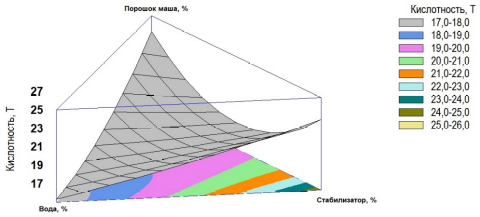
\includegraphics[width=0.7\textwidth]{media/pish/image5}
	\caption*{Figure 1 - Response Surface of the Output Parameter: Dependence
of Acidity on the Mass Fraction of Components}
\end{figure}

Thus, the dependence of acidity on the components of plant-based milk
from mung beans can be represented in terms of the mass fraction of the
ingredients individually, and the regression equation can be written in
the following form (formula 1):

\begin{equation}
y = 25,2714x_1 + 17,3143x_2+ 24,6143x_3- 6,04284x_1x_2- 20,4428x_1x_3- 1,41427x2x_3
\end{equation}

Based on the obtained regression equation, a model was constructed in
three-dimensional space, representing a plane that characterizes the
dependence of acidity on the components of plant-based milk.

Figures 1-4 present graphical representations of the dependency plots.

\begin{figure}[H]
	\centering
	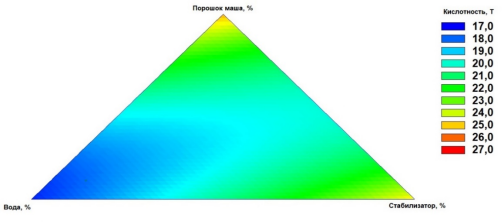
\includegraphics[width=0.7\textwidth]{media/pish/image6}
	\caption*{Figure 2 - Projections of the Response Surface Sections
Characterizing the Dependence of Acidity on the Mass Fraction of
Components}
\end{figure}

\begin{figure}[H]
    \centering
    \begin{subfigure}[t]{0.44\textwidth} % Align at the top
        \centering
        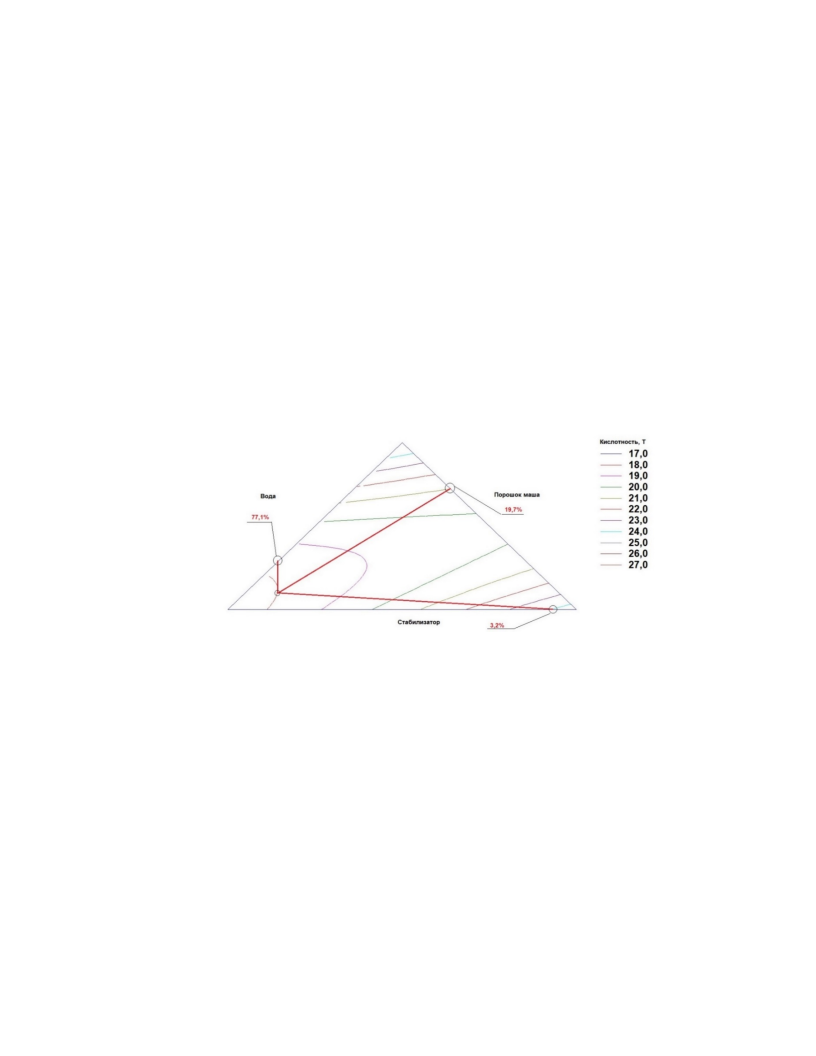
\includegraphics[width=\textwidth]{media/pish/image7}
        \caption*{Figure 3 - Projections of the Response Surface Sections
Characterizing the Dependence of Acidity on the Mass Fraction of
Components with Optimal Points}
    \end{subfigure}
    \hspace{0.05\textwidth} % Adjust horizontal space between the subfigures
    \begin{subfigure}[t]{0.44\textwidth} % Align at the top
        \centering
        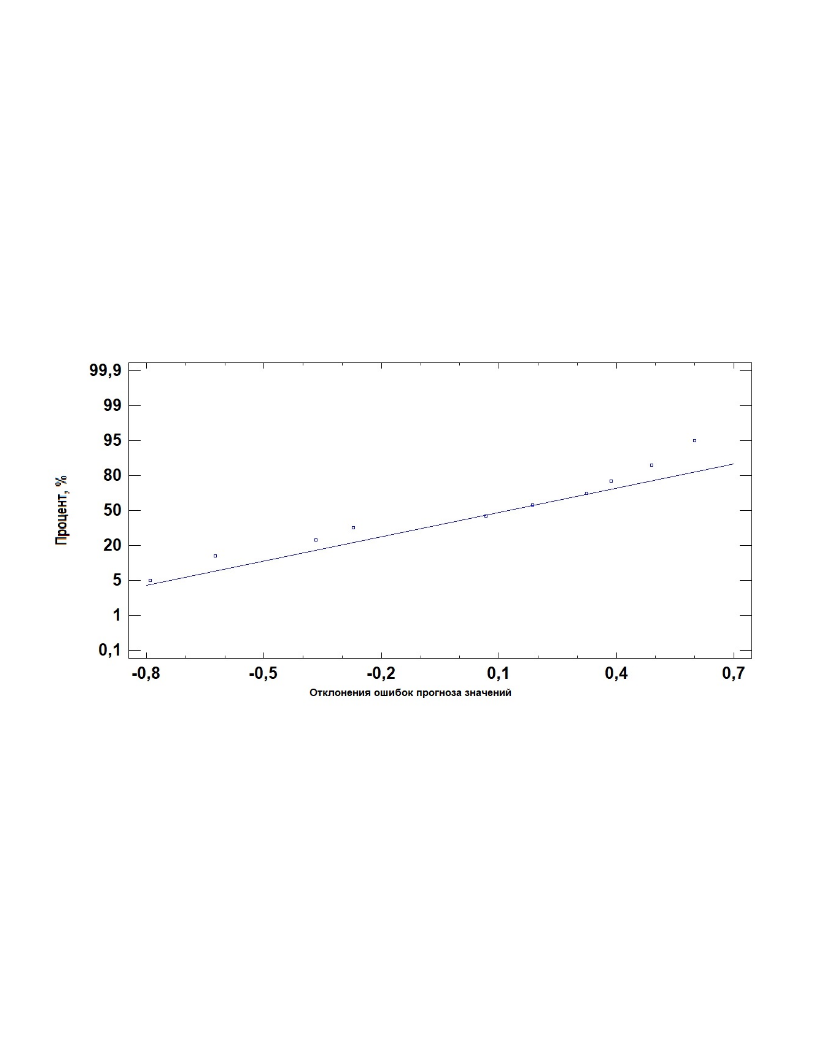
\includegraphics[width=\textwidth]{media/pish/image8}
        \caption*{Figure 4 - Diagnostic Plot of the Deviation of Predicted Acidity
Values from Normal Distribution}
    \end{subfigure}
\end{figure}

\begin{multicols}{2}
The analysis of the behavior of the obtained response surface showed
that the optimal zone for the acidity of plant-based milk is achieved
when the mass fraction of mung bean powder is 19.7\%, the mass fraction
of water is 77.1\%, and the mass fraction of stabilizer is 3.2\%. The
analysis of the distribution of errors in predicting acidity values
yielded satisfactory results: a significant portion of the points did
not deviate noticeably from the line, indicating the adequacy of the
obtained model.

{\bfseries Conclusion.} Mung beans are a widely recognized plant-based
source of protein and a means of maintaining health due to their high
nutrient content. Currently, people' s demands for
quality of life are continuously improving, while simultaneously, the
prevalence of unhealthy populations is steadily rising. The "generation
of people who eat medicines" is gradually being perceived by consumers
as a whole.

\emph{{\bfseries Funding:} This research was funded by the Ministry of
Agriculture of the Republic of Kazakhstan (BR22886613).}
\end{multicols}

\begin{center}
{\bfseries References}
\end{center}

\begin{references}
1. Merenkova S.P., Androsova N.V. Aktual' nye aspekty
proizvodstva napitkov na rastitel' nom
syr' e // Vestnik YUUrGU. Seriya «Pishchevye i
biotekhnologii». - 2018. - T.6. - № 3. - S. 57-67. DOI:
\\10.14529/food180307. {[}In Russian{]}

2. Egorova S.V., Ahmatziaeva M.M., Rostegaev R.S.
Rastitel' naya pishcha budushchego // V sbornike:
Advanced science: sbornik statej III Mezhdunarodnoj
nauchno-prakticheskoj konferencii: v 2 ch. - 2018. - S.134-137. {[}In
Russian{]}

3. Kazakov I.O., Kiseleva T.F., Eremina I.A., Mikova D.S. Issledovaniya
vliyaniya ul' trazvukovoj obrabotki na
stojkost'{} napitkov na osnove zernovogo
syr' ya // Food Processing: Techniques and Technology. -
№ 1. - 2015. - S. 30-34. {[}In Russian{]}

4. Mayuri Chavan, Yogesh Gat, Mugdha Harmalkar, Roji Waghmare.
Development of nondairy

fermented probiotic drink based on germinated and ungerminated cereals
and legume // LWT -Food Science and Technology. - 2018. - Vol. 91. - Р.
339-344. DOI: 10.1016/j.lwt.2018.01.070

5. Mridula D. Monika Sharma. Development of non-dairy probiotic drink
utilizing sprouted cereals, legume and soymilk // LWT -- Food Science
and Technology. - 2015. - vol. 62. - Р. 482-487. DOI:
\\10.1016/j.lwt.2014.07.011

6. Pasquale Russo, Maria Lucia, Valeria de Chiara et al. Lactobacillus
plantarum strains for multifunctional oat-based foods // LWT -- Food
Science and Technology. - 2015. - vol. 68. - Р. 288 -294. DOI:
\\10.1016/j.lwt.2015.12.040

7. Mradula Gupta, Somesh Sharma. Probiotics in limelight // Journal of
Innovative Biology. - 2016. - vol. 3. - Р. 276-280.

8. Loh W. The epidemiology of food allergy in the global context Int. //
J. Environ. Res. Public Health. -- 2018. -- 15. -- 2043.
DOI:10.3390/ijerph15092043

9. Muhammad Iqbal, Nadiah Zafar, Hatem Fessi, Abdelhamid Elaissari
Double emulsion solvent evaporation techniques used for drug
encapsulation // International Journal of Pharmaceutics. -- 2015. -
Volume 496. - Р. 173-190. DOI:10.1016/j.ijpharm.2015.10.057

10. Rajan A. Production of soya milk containing low flatulence-causing
oligosaccharides in a packed bed reactor using immobilised
α-galactosidase: Immobilised α-galactosidase // International Journal of
Food Science \& Technology. - 2010. - V. 45. - № 10. - Р. 2023-2031.
DOI:10.1111/j.1365- 2621.2010.02354.x.
\end{references}

\begin{authorinfo}
\hspace{1em}\emph{{\bfseries Information about the authors}}

N.Alzhaxina - PhD, Director of the Astana branch of «Kazakh Research
Institute of Processing and Food Industry», Astana, Kazakhstan, e-mail:
\href{mailto:alzhaxina@inbox.ru}{\nolinkurl{alzhaxina@inbox.ru}};

I. Aubakirova - Master' s student, Junior researcher,
Astana branch of «Kazakh Research Institute of Processing and Food
Industry», Astana, Kazakhstan, е-mail: aubakirova.inkar@bk.ru.

\hspace{1em}\emph{{\bfseries Информация об авторах}}

Альжаксина Н.E. - PhD, и.о. директора Астанинского филиала ТОО
«Казахский научно-исследовательский институт перерабатывающей и пищевой
промышленности», Астана, Казахстан, е-mail:
\href{mailto:alzhaxina@inbox.ru}{\nolinkurl{alzhaxina@inbox.ru}};

Аубакирова И.Е. - магистрант, младший научный сотрудник Астанинского
филиала ТОО «Казахский научно-исследовате-льский институт
перерабатывающей и пищевой промышленности», Астана, Казахстан, е-mail:
aubakirova.inkar@bk.ru.
\end{authorinfo}
